\documentclass{article}
\usepackage[utf8]{inputenc}
\usepackage{polski}
\usepackage{geometry}
\usepackage{pdfpages}
\usepackage{pdfpages}
\usepackage{listings}
\usepackage{listingsutf8}
\usepackage{multirow}
\usepackage{siunitx}
\usepackage{booktabs}
\usepackage{tabularx}
\usepackage{placeins}
\usepackage{pdflscape}

\geometry{
a4paper,
total={170mm,257mm},
left=20mm,
top=20mm
}
\newcolumntype{Y}{>{\centering\arraybackslash}X}
% \renewcommand\thesection{}
\lstset{%
literate=%
 {ą}{{\k{a}}}1
 {ę}{{\k{e}}}1
 {Ą}{{\k{A}}}1
 {Ę}{{\k{E}}}1
 {ś}{{\'{s}}}1
 {Ś}{{\'{S}}}1
 {ź}{{\'{z}}}1
 {Ź}{{\'{Z}}}1
 {ń}{{\'{n}}}1
 {Ń}{{\'{N}}}1
 {ć}{{\'{c}}}1
 {Ć}{{\'{C}}}1
 {ó}{{\'{o}}}1
 {Ó}{{\'{O}}}1
 {ż}{{\.{z}}}1
 {Ż}{{\.{Z}}}1
 {ł}{{\l{}}}1
 {Ł}{{\l{}}}1
}

\title{Technika Cyfrowa\\
Sprawozdanie - bramki logiczne}
\author{Maciej Trątnowiecki}
\date{AGH, Semestr Letni, 2020}

\begin{document}
    \maketitle
    \section{Układ sumujący dwie liczby trzybitowe}
        \subsection{Realizowana funkcja logiczna}
            Układ ma trzy wejścia, ABC odpowiadające za bity pierwszej z liczb i DEF odpowiadające za bity drugiej, oraz cztery wyjścia GHIJ.
            Gdy sumujemy pojedyńczą parę bitów, możemy otrzymać cztery sytuacje opisane poniższą tabelą prawdy. 
            \begin{center}
                \begin{table}[ht]
                    \centering
                    \begin{tabular}{|c|c|c|}
                        \hline
                        C & F & J\\
                        \specialrule{1pt}{1pt}{1pt}
                        0 & 0 & 0\\
                        \hline
                        0 & 1 & 1\\
                        \hline
                        1 & 0 & 1\\
                        \hline
                        1 & 1 & 0\\
                        \hline 
                    \end{tabular}
                    \caption{Tabela prawdy dla sumy dwóch bitów.}
                    \label{tab:my_label}
                \end{table}
            \end{center}
            W ostatniej sytuacji, gdy oba sumowane bity miały stan wysoki otrzymaliśmy zero. Jednak powinniśmy otrzymać dwa w zapisie dziesiętnym, to jest 10 w zapisie binarnym. Dzieje się tak dlatego, że w tabeli przewidzieliśmy zaledwie pojedyncze wyjście. Nastąpiło tak zwane przepełnienie, to znaczy otrzymana liczba nie daje się reprezentować w przewidzianym zakresie bitów. Zostanie on zatem rozszerzony do dwóch bitów. 
            \begin{center}
                \begin{table}[ht]
                    \centering
                    \begin{tabular}{|c|c|c|}
                        \hline
                        C & F & IJ\\
                        \specialrule{1pt}{1pt}{1pt}
                        0 & 0 & 00\\
                        \hline
                        0 & 1 & 01\\
                        \hline
                        1 & 0 & 01\\
                        \hline
                        1 & 1 & 10\\
                        \hline 
                    \end{tabular}
                    \caption{Tabela prawdy dla sumy dwóch bitów.}
                    \label{tab:my_label}
                \end{table}
            \end{center}
            W powyższej tabeli wyjście J odpowiada za wynik sumowania, a wyjście I za informację o przepełnieniu. Możemy ich wartości opisać poniższymi tabelami. 
            \begin{center}
                \begin{table}[ht]
                    \centering
                    \begin{tabular}{|c|c|c|}
                        \hline
                        C / F & 0 & 1\\
                        \hline
                        0 & 0 & 1\\
                        \hline
                        1 & 1 & 0\\
                        \hline
                    \end{tabular}
                    \caption{Tabela prawdy dla wyjścia J (wynik dodawania).}
                    \label{tab:my_label}
                \end{table}
            \end{center}
            \begin{center}
                \begin{table}[ht]
                    \centering
                    \begin{tabular}{|c|c|c|}
                        \hline
                        C / F & 0 & 1\\
                        \hline
                        0 & 0 & 0\\
                        \hline
                        1 & 0 & 1\\
                        \hline
                    \end{tabular}
                    \caption{Tabela prawdy dla wyjścia I (informacja o przepełnieniu).}
                    \label{tab:my_label}
                \end{table}
            \end{center}
            Z powyższych tabel odczytać możemy zależności opisujące stany na tych wyjściach.
            $$I = FC$$
            $$J = F\overline{C} + \overline{F}C = F\oplus C$$
            
            Sumując liczby dwubitowe, będziemy musieli rozpatrzyć wynik z poprzedniej pary bitów. Oznacza to, że będziemy musieli rozpatrzyć trzy bity na wejściu. Tabelę prawdy takiej operacji przedstawiono poniżej. Małym i oznaczono przepełnienie z sumy poprzedniej pary bitów.
            \begin{center}
                \begin{table}[ht]
                    \centering
                    \begin{tabular}{|c|c|c|c|}
                        \hline
                        B & E & i & HI\\
                        \specialrule{1pt}{1pt}{1pt}
                        0 & 0 & 0 & 00\\
                        \hline
                        0 & 0 & 1 & 01\\
                        \hline
                        0 & 1 & 0 & 01\\
                        \hline
                        0 & 1 & 1 & 10\\
                        \hline
                        1 & 0 & 0 & 01\\
                        \hline
                        1 & 0 & 1 & 10\\
                        \hline
                        1 & 1 & 0 & 10\\
                        \hline
                        1 & 1 & 1 & 11\\
                        \hline 
                    \end{tabular}
                    \caption{Tabela prawdy dla sumy dwóch bitów.}
                    \label{tab:my_label}
                \end{table}
            \end{center}
            Dla takiej sumy również zapiszemy zależności konkretnych wyjść. 
            % \begin{center}
            %     \begin{table}[ht]
            %         \centering
            %         \begin{tabular}{|c|c|c|c|c|}
            %             \hline
            %             B / Ei & 00 & 01 & 11 & 10 \\
            %             \hline
            %             0 & 0 & 1 & 0 & 1\\
            %             \hline
            %             1 & 1 & 0 & 1 & 0\\
            %             \hline
            %         \end{tabular}
            %         \caption{Tabela prawdy dla wyjścia I (wynik dodawania).}
            %         \label{tab:my_label}
            %     \end{table}
            % \end{center}
            % \begin{center}
            %     \begin{table}[ht]
            %         \centering
            %         \begin{tabular}{|c|c|c|c|c|}
            %             \hline
            %             B / Ei & 00 & 01 & 11 & 10 \\
            %             \hline
            %             0 & 0 & 0 & 1 & 0\\
            %             \hline
            %             1 & 0 & 1 & 1 & 1\\
            %             \hline
            %         \end{tabular}
            %         \caption{Tabela prawdy dla wyjścia H (informacja o przepełnieniu).}
            %         \label{tab:my_label}
            %     \end{table}
            % \end{center}
            \begin{center}
                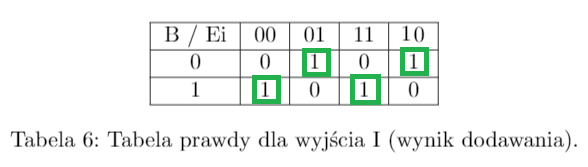
\includegraphics[widht=18cm]{reports/img/Z1A_tab_1.png}\\
            \end{center}
            \begin{center}
                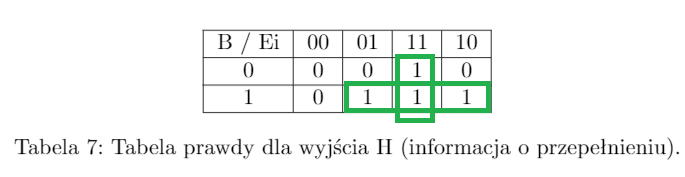
\includegraphics[widht=18cm]{reports/img/Z1A_tab_2.png}\\
            \end{center}
            Skąd otrzymujemy poniższe zależności. 
            $$I = B\overline{E}\overline{i} + \overline{B}\overline{E}i + BEi + \overline{B}E\overline{i} = B(\overline{E}\overline{i} + Ei) + \overline{B}(\overline{E}i + E\overline{i}) = \overline{B}(E\oplus i) + B(\overline{(E\oplus i)}) = B\oplus E\oplus i$$
            $$H = Ei + B(E + i) = Ei + BE + Bi$$



        \subsection{Sumator pełny i pół-pełny}
            Dla sumy najmniej ważnych bitów na wejściu sumatora otrzymujemy dwa sygnały - po jednym bicie od każdej z liczb. Jednakże, wynik dodawania dwóch liczb jednobitowych jest liczbą dwubitową. Dlatego, na wyjściu podajemy dwa sygnały - stan najmniej ważnego bitu liczby wynikowej i informacje o tym, czy wystąpiło przepełnienie.\\
            Taki układ nazywamy sumatorem pół-pełnym, jednobitowym. Do jego wykonania wykorzystano dwie bramki logiczne - xor i and, do których podłączymy sygnały wejściowe. Wyjście bramki xor będzie stanem bitu w wyniku, a wyjście bramki and informacją o przepełnieniu. \\
            \begin{figure}[h!]
                \centering
                
\includegraphics[width=13cm]{reports/img/Z1A_polpelny.png}
                \caption{Sumator pół-pełny}
            \end{figure}\\
            \FloatBarrier
            Podczas sumowania kolejnych bitów będziemy musieli rozpatrzyć trzy sygnały wejściowe - dwa jak poprzednio informujące o wartościach bitów w dodawanej liczbie, a trzeci informujący czy w poprzedniej operacji dodawania wystąpiło przepełnienie. Na wyjściu ponownie znajdą się dwa sygnały - jak w sumatorze pół-pełnym.\\
            Układ realizujący taką sumę nazywamy sumatorem pełnym.
            \begin{figure}[h!]
                \centering
                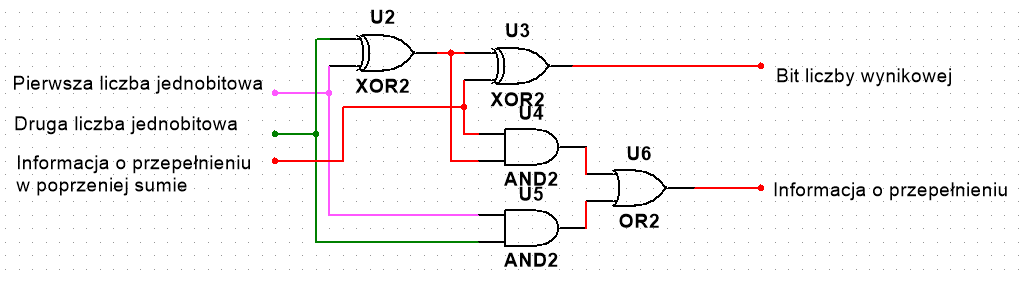
\includegraphics[width=13cm]{reports/img/Z1A_pelny.png}
                \caption{Sumator pełny}
            \end{figure}\\
            \FloatBarrier
        
        \subsection{Konstrukcja układu sumującego}
            Zauważmy, że tak skonstruowane sumatory pełne można dowolnie długo łączyć, otrzymując na ich wyjściach poprawną sumę arytmetyczną liczb przekazanych na wejścia. W celu ograniczenia ilości użytych bramek logicznych do wykonania sumy najmniej znaczących bitów używamy sumatora pół-pełnego.\\ 
            Aby wykonać sumę dwóch liczb trzybitowych potrzeba dwóch sumatorów pełnych i jednego pół-pełnego.

        \subsection{Projekt układu}
            \begin{center}
                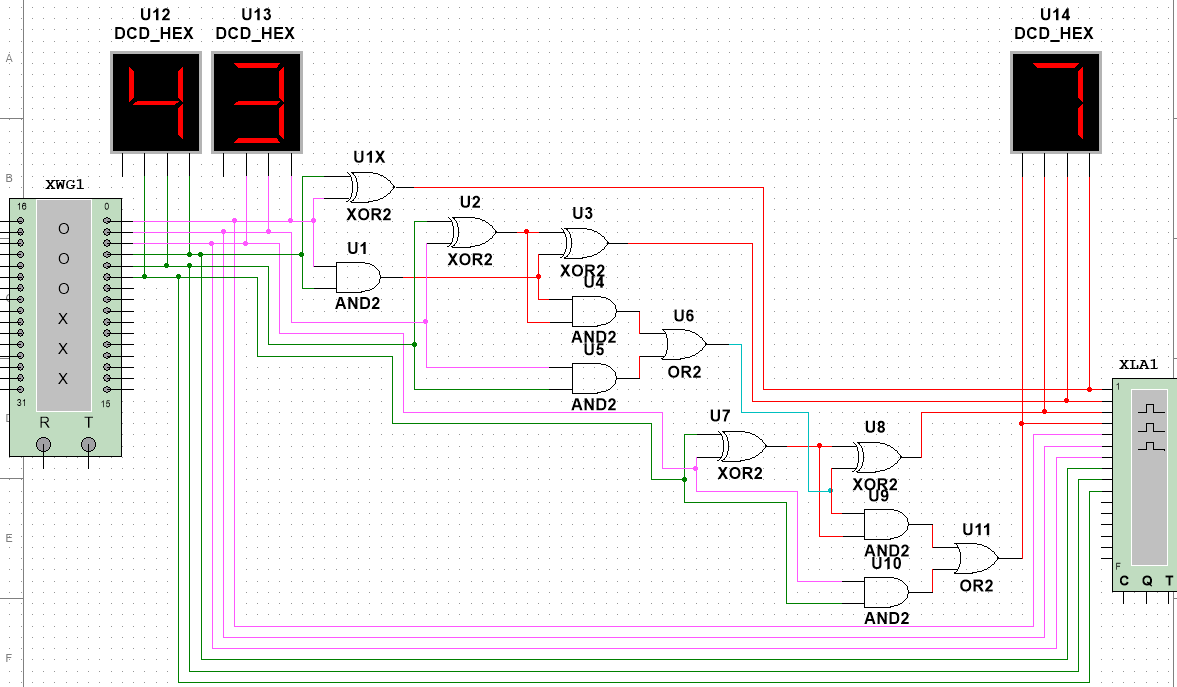
\includegraphics[height=9cm]{reports/img/Z1A_1.png}\\
            \end{center}
            W układzie jako źródło sygnału wykorzystano generator słów. Wyjścia odpowiadające za bity pierwszej z liczb oznaczono kolorem zielonym, a za bity drugiej z nich kolorem różowym. \\
            Do obliczenia sumy arytmetycznej wykorzystano jeden sumator pół-pełny (dla sumy najmniej ważnych bitów), oraz dwa sumatory pełne. Wyjścia odpowiadające za przepełnienie oznaczono kolorem lazurowym. \\
            Wynik operacji zilustrowano poprzez wykorzystanie wyświetlacza HEX. 
        
        \subsection{Symulacja}
            W celu przetestowania układu dla wszystkich par liczba trzybitowych generator ustawiony został w tryb generowania wszystkich liczb sześciobitowych od $111111$ do $000000$. Trzy najmniej znaczące bity odpowiadają za jedną z generowanych liczb, trzy najmniej znaczące za drugą.   
            \begin{center}
                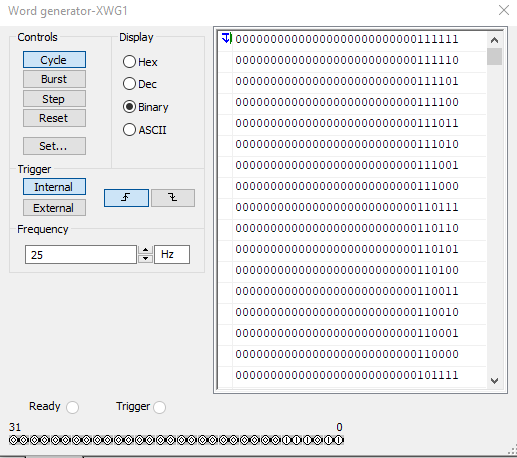
\includegraphics[height=9cm]{reports/img/Z1A_gen.png}\\
            \end{center}
            \begin{center}
                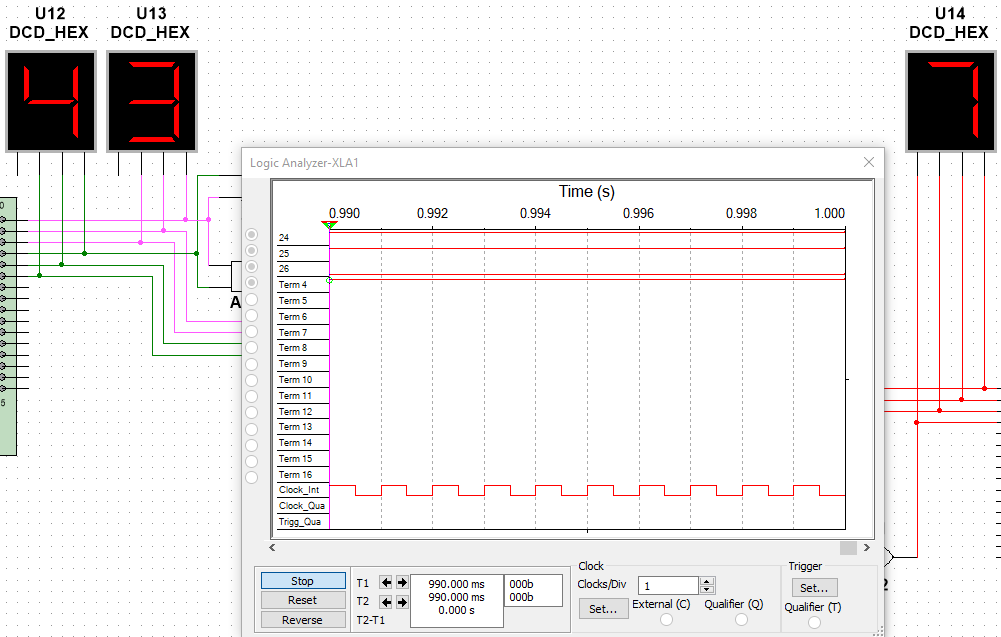
\includegraphics[height=9cm]{reports/img/Z1A_analize.png}\\
            \end{center}
            Z ekranu analizatora logicznego odczytać możemy wynikową liczbę czterobitową, oraz trzybitowe liczby wejściowe od których jest zależna. Na tej podstawie możemy stwierdzić poprawność implementacji.

            
        \subsection{Wnioski}
            Zauważmy, że w przedstawiony powyżej sposób możemy niskim kosztem skonstruować sumator dla dwóch liczb o dowolnej (choć z góry ustalonej) liczby bitów. Taki układ może znaleźć zastosowanie w wielu sytuacjach codziennych. Dla przykładu, w układzie sterowania moją pralką. Na tryb prania składa się wiele etapów, jak moczenie, pranie, czy wirowanie. Długość każdego z tych etapów zależy od wybranych parametrów (jak temperatura wody, czy ocena stopnia zabrudzenia ubrań). Na wyświetlaczu pokazuje ona sumaryczny czas prania, będący w istocie sumą po czasach trwania każdego z tych etapów. Możemy zatem zastosować przygotowany powyżej sumator do obliczenia liczby przekazywanej na wejścia dekodera wyświetlacza. 
            
            
    \section{Układ sprawdzający równość dwóch liczb}
        \subsection{Konstrukcja układu}
            Układ komparatora dwóch liczb czterobitowych ma cztery wejścia, ABCD odpowiadające za bity pierwszej z liczb i EFGH odpowiadające za bity drugiej. Chcemy zrealizować funkcję logiczną 
            $$(A==E)\land(B==F)\land(C==G)\land(D==H)$$
            Co jest równoważne z
            $$(\neg(A\oplus E))\land(\neg(B\oplus F))\land(\neg(C\oplus G))\land(\neg(D\oplus H))$$
            $$\neg((A\oplus E)\lor(B\oplus F)\lor(C\oplus G)\lor(D\oplus H))$$
            Zatem w celu wykazania ich równości, wystarczy zastosować bramki XOR w ilości odpowiadającej liczbie bitów, których wyjścia zestawić należy bramką NOR. 

        \subsection{Projekt układu}
            \begin{center}
                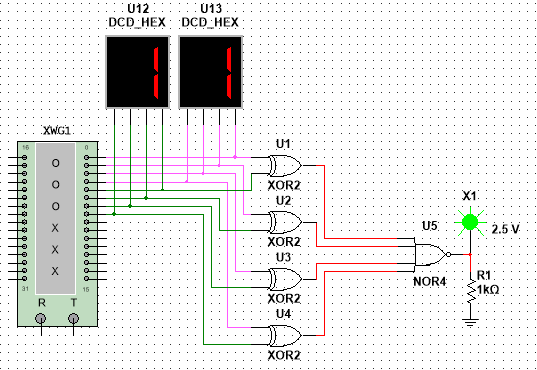
\includegraphics[height=9cm]{reports/img/Z1B_1.png}\\
            \end{center}
            W układzie jako źródło sygnału wykorzystano generator słów. Wyjścia odpowiadające za bity pierwszej z liczb oznaczono kolorem zielonym, a za bity drugiej z nich kolorem różowym. \\
            Do porównania wartości liczb wykorzystano bramki xor, których wyniki zbiera bramka nor. \\
            Równość liczb sygnalizuje zielona dioda. 
            \FloatBarrier
            
        \subsection{Wnioski}
            Zauważmy, że w przedstawiony powyżej sposób możemy skonstruować układ sprawdzający równość  dwóch liczb o dowolnej (choć z góry ustalonej) liczbie bitów. Domofon wejściowy w bloku w którym mieszkam można otworzyć wprowadzając specjalny kod mający postać liczby naturalnej. Za porównanie go z przewidzianą w układzie sekwencją bitów odpowiadać może układ podobny do przedstawionego powyżej. 

    \section{Transkoder czterobitowych cyfr szesnastkowych na wyświetlacz siedmiosegmentowy}
        \subsection{Minimalizacja funkcji boolowskich}
            Wyświetlaczem sterować można poprzez 7 wyjść, ponumerowanych od A do G, każde z nich odpowiada za inny segment wyświetlacza. W poniższej tabeli zebrano opis ustawień wyjść odpowiedzialnych za wyświetlanie każdej z liczb czterobitowych.
            \newpage
            \begin{center}
                \begin{table}[ht]
                    \centering
                    \begin{tabularx}{\textwidth}{|c|c| *{7}{Y|}} %{|c|c|c|c|c|c|c|c|c|}
                        \hline
                        % \multirow{ 2}{*}{Liczba w systemie szesnastkowym} &  
                        % \multirow{ 2}{*}{Liczba w systemie binarnym} &
                        \textbf{Liczba w systemie} & \textbf{Liczba w systemie} &
                        \multicolumn{7}{|l|}{\textbf{Wyjścia wyświetlacza siedmiosegmentowego}}\\
                        \cline{3-9}
                        \textbf{szesnastkowym} & \textbf{binarnym} & \textbf{A} & \textbf{B} & \textbf{C} & \textbf{D} & \textbf{E} & \textbf{F} & \textbf{G} \\
                        \specialrule{.1em}{.05em}{.05em} 
                         0 & 0000 & 1 & 1 & 1 & 1 & 1 & 1 & 0\\
                        %  \hline 
                         1 & 0001 & 0 & 1 & 1 & 0 & 0 & 0 & 0\\
                        %  \hline 
                         2 & 0010 & 1 & 1 & 0 & 1 & 1 & 0 & 1\\
                        %  \hline 
                         3 & 0011 & 1 & 1 & 1 & 1 & 0 & 0 & 1\\
                        %  \hline 
                         4 & 0100 & 1 & 1 & 1 & 0 & 0 & 1 & 1\\
                        %  \hline 
                         5 & 0101 & 1 & 0 & 1 & 1 & 0 & 1 & 1\\
                        %  \hline 
                         6 & 0110 & 1 & 0 & 1 & 1 & 1 & 1 & 1\\
                        %  \hline 
                         7 & 0111 & 1 & 1 & 1 & 0 & 0 & 0 & 0\\
                        %  \hline 
                         8 & 1000 & 1 & 1 & 1 & 1 & 1 & 1 & 1\\
                        %  \hline 
                         9 & 1001 & 1 & 1 & 1 & 0 & 0 & 1 & 1\\
                        %  \hline
                         A & 1010 & 1 & 1 & 1 & 0 & 1 & 1 & 1\\
                        %  \hline
                         B & 1011 & 0 & 0 & 1 & 1 & 1 & 1 & 1\\ 
                        %  \hline
                         C & 1100 & 1 & 0 & 0 & 1 & 1 & 1 & 0\\
                        %  \hline
                         D & 1101 & 0 & 1 & 1 & 1 & 1 & 0 & 1\\
                        %  \hline
                         E & 1110 & 1 & 0 & 0 & 1 & 1 & 1 & 1\\
                        %  \hline
                         F & 1111 & 1 & 0 & 0 & 0 & 1 & 1 & 1\\
                        \hline
                    \end{tabularx}
                    \caption{Wyjścia wyświetlacza}
                    \label{tab:my_label}
                \end{table}
            \end{center}
            W celu uproszczenia układu wykonać należy minimalizację metodą Karnaugh dla każdego z wyjść wyświetlacza. Niech $x_1, x_2, x_4, x_8$ określają kolejne bity, czterobitowej liczby $x$ w kolejności od najmniej do najbardziej znaczącego bitu. Wtedy:
            \begin{center}
                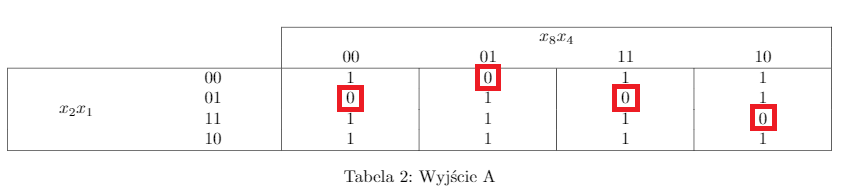
\includegraphics[width=18cm]{reports/img/Z1C_tab_1.png}\\
            \end{center}

            % \begin{center}
            %     \begin{table}
            %         \centering
            %         \begin{tabularx}{\textwidth}{|Y *{5}{Y|}}
            %             \cline{3-6} 
            %             \multicolumn{2}{c|}{} &
            %             \multicolumn{4}{c|}{$x_8x_4$}\\
                        
            %             \multicolumn{2}{c|}{} & \multicolumn{1}{c}{00} & \multicolumn{1}{c}{01} & \multicolumn{1}{c}{11} & \multicolumn{1}{c|}{10}\\
            %             \hline
                         
            %             \multirow{4}{*}{$x_2x_1$} & 00 & 1 & 0 & 1 & 1 \\
            %                                       & 01 & 0 & 1 & 0 & 1 \\
            %                                       & 11 & 1 & 1 & 1 & 0 \\
            %                                       & 10 & 1 & 1 & 1 & 1 \\
                        
            %              \hline 
            %         \end{tabularx}
            %         \caption{Wyjście A}
            %         \label{tab:my_label}
            %     \end{table}
            % \end{center}

            Zauważmy, że wartości zera logicznego w powyższej tabeli jest zdecydowanie mniej, niż stanów wysokich. Dlatego to po nich będziemy grupować, zatem otrzymamy wynik poprzez dopełnienie.\\
            Każdą z grup zer możemy opisać poprzez określenie w postaci alternatywy logicznej wszystkich pozostałych wartości w tablicy, za wyjątkiem tej grupy. Taką grupę konstruujemy poprzez negację logiczną. Jeśli na tak przygotowanych grupach użyjemy koniunkcji logicznej otrzymamy formułę opisującą poprawnie rozkład stanów wysokich i niskich względem sygnału wejściowego dla danego wejścia wyświetlacza. \\
            Skąd otrzymujemy (przez dopełnienie):
            $$A = (\overline{x_1}+x_2+x_4+x_8)(x_1+x_2+\overline{x_4}+x_8)(\overline{x_1}+x_2+\overline{x_4}+\overline{x_8})(\overline{x_1}+\overline{x_2}+x_4+\overline{x_8})$$
            Analogiczną analizę przeprowadzimy dla każdego z pozostałych wejść wyświetlacza.
            \begin{center}
                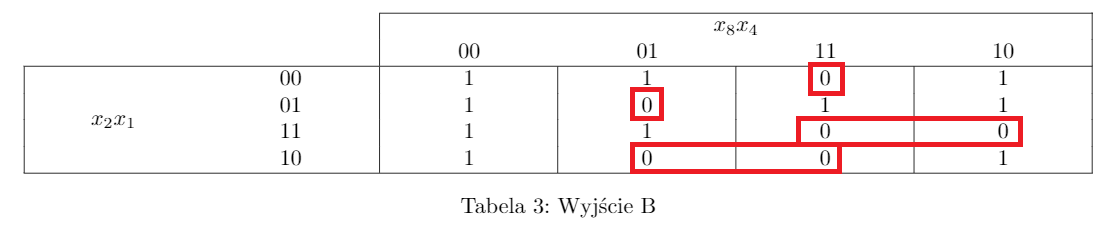
\includegraphics[width=18cm]{reports/img/Z1C_tab_3.png}\\
            \end{center}
            % \begin{center}
            %     \begin{table}[ht]
            %         \centering
            %         \begin{tabularx}{\textwidth}{|Y *{5}{Y|}}
            %             \cline{3-6} 
            %             \multicolumn{2}{c|}{} &
            %             \multicolumn{4}{c|}{$x_8x_4$}\\
                        
            %             \multicolumn{2}{c|}{} & \multicolumn{1}{c}{00} & \multicolumn{1}{c}{01} & \multicolumn{1}{c}{11} & \multicolumn{1}{c|}{10}\\
            %             \hline
                         
            %             \multirow{4}{*}{$x_2x_1$} & 00 & 1 & 1 & 0 & 1 \\
            %                                       & 01 & 1 & 0 & 1 & 1 \\
            %                                       & 11 & 1 & 1 & 0 & 0 \\
            %                                       & 10 & 1 & 0 & 0 & 1 \\
                        
            %              \hline 
            %         \end{tabularx}
            %         \caption{Wyjście B}
            %         \label{tab:my_label}
            %     \end{table}
            % \end{center}
            \FloatBarrier
            Skąd otrzymujemy (przez dopełnienie):
            $$ B = (\overline{x_1}+x_2+\overline{x_4}+x_8)(\overline{x_1}+\overline{x_2}+\overline{x_8})(x_1+x_2+\overline{x_4}+\overline{x_8})(x_1+\overline{x_2}+\overline{x_4})$$
            \begin{center}
                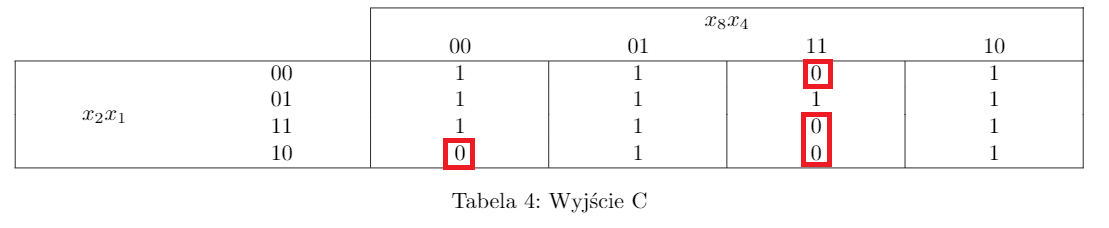
\includegraphics[width=18cm]{reports/img/Z1C_tab_4.png}\\
            \end{center}
            % \begin{center}
            %     \begin{table}[ht]
            %         \centering
            %         \begin{tabularx}{\textwidth}{|Y *{5}{Y|}}
            %             \cline{3-6} 
            %             \multicolumn{2}{c|}{} &
            %             \multicolumn{4}{c|}{$x_8x_4$}\\
                        
            %             \multicolumn{2}{c|}{} & \multicolumn{1}{c}{00} & \multicolumn{1}{c}{01} & \multicolumn{1}{c}{11} & \multicolumn{1}{c|}{10}\\
            %             \hline
                         
            %             \multirow{4}{*}{$x_2x_1$} & 00 & 1 & 1 & 0 & 1 \\
            %                                       & 01 & 1 & 1 & 1 & 1 \\
            %                                       & 11 & 1 & 1 & 0 & 1 \\
            %                                       & 10 & 0 & 1 & 0 & 1 \\
                        
            %              \hline 
            %         \end{tabularx}
            %         \caption{Wyjście C}
            %         \label{tab:my_label}
            %     \end{table}
            % \end{center}
            \FloatBarrier
            Skąd otrzymujemy (przez dopełnienie):
            $$C = (x_1+\overline{x_2}+x_4+x_8)(\overline{x_2}+\overline{x_4}+\overline{x_8})(x_1+x_2+\overline{x_4}+\overline{x_8})$$
            \begin{center}
                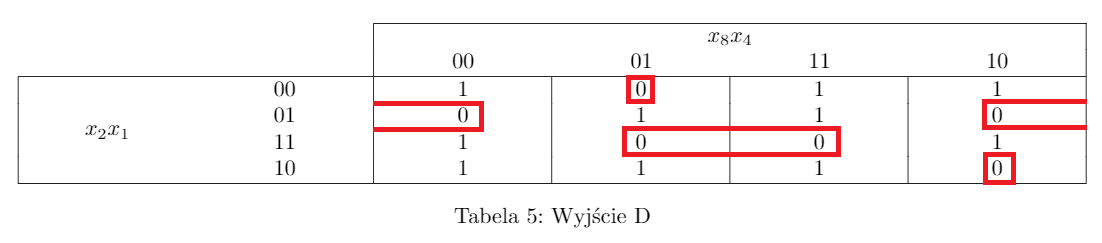
\includegraphics[width=18cm]{reports/img/Z1C_tab_5.png}\\
            \end{center}
            % \begin{center}
            %     \begin{table}[ht]
            %         \centering
            %         \begin{tabularx}{\textwidth}{|Y *{5}{Y|}}
            %             \cline{3-6} 
            %             \multicolumn{2}{c|}{} &
            %             \multicolumn{4}{c|}{$x_8x_4$}\\
                        
            %             \multicolumn{2}{c|}{} & \multicolumn{1}{c}{00} & \multicolumn{1}{c}{01} & \multicolumn{1}{c}{11} & \multicolumn{1}{c|}{10}\\
            %             \hline
                         
            %             \multirow{4}{*}{$x_2x_1$} & 00 & 1 & 0 & 1 & 1 \\
            %                                       & 01 & 0 & 1 & 1 & 0 \\
            %                                       & 11 & 1 & 0 & 0 & 1 \\
            %                                       & 10 & 1 & 1 & 1 & 0 \\
                        
            %              \hline 
            %         \end{tabularx}
            %         \caption{Wyjście D}
            %         \label{tab:my_label}
            %     \end{table}
            % \end{center}
            \FloatBarrier
            Skąd otrzymujemy (przez dopełnienie):
            $$D = (x_1+x_2+\overline{x_4}+x_8)(\overline{x_1}+x_2+x_4)(\overline{x_1}+\overline{x_2}+\overline{x_4})(x_1+\overline{x_2}+x_4+\overline{x_8})$$
            \begin{center}
                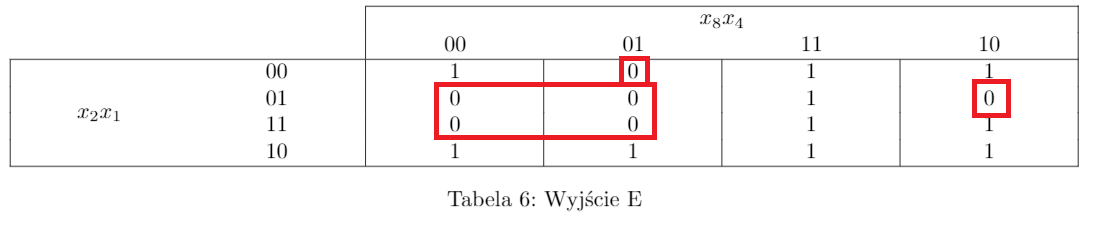
\includegraphics[width=18cm]{reports/img/Z1C_tab_6.png}\\
            \end{center}
            % \begin{center}
            %     \begin{table}[ht]
            %         \centering
            %         \begin{tabularx}{\textwidth}{|Y *{5}{Y|}}
            %             \cline{3-6} 
            %             \multicolumn{2}{c|}{} &
            %             \multicolumn{4}{c|}{$x_8x_4$}\\
                        
            %             \multicolumn{2}{c|}{} & \multicolumn{1}{c}{00} & \multicolumn{1}{c}{01} & \multicolumn{1}{c}{11} & \multicolumn{1}{c|}{10}\\
            %             \hline
                         
            %             \multirow{4}{*}{$x_2x_1$} & 00 & 1 & 0 & 1 & 1 \\
            %                                       & 01 & 0 & 0 & 1 & 0 \\
            %                                       & 11 & 0 & 0 & 1 & 1 \\
            %                                       & 10 & 1 & 1 & 1 & 1 \\
                        
            %              \hline 
            %         \end{tabularx}
            %         \caption{Wyjście E}
            %         \label{tab:my_label}
            %     \end{table}
            % \end{center}
            \FloatBarrier
            Skąd otrzymujemy (przez dopełnienie):
            $$E = (\overline{x_1}+x_8)(x_1+x_2+\overline{x_4}+x_8)(\overline{x_1}+x_2+x_4+\overline{x_8})$$
            \begin{center}
                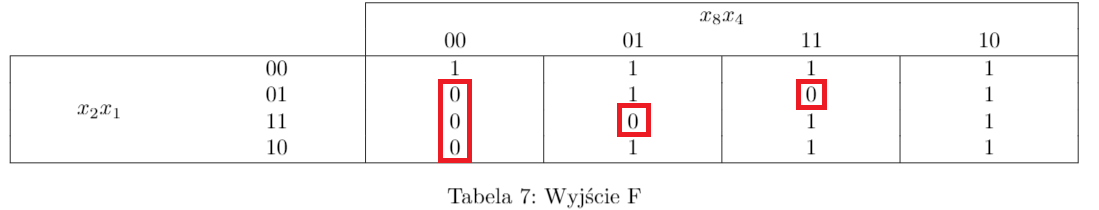
\includegraphics[width=18cm]{reports/img/Z1C_tab_7.png}\\
            \end{center}
            % \begin{center}
            %     \begin{table}[ht]
            %         \centering
            %         \begin{tabularx}{\textwidth}{|Y *{5}{Y|}}
            %             \cline{3-6} 
            %             \multicolumn{2}{c|}{} &
            %             \multicolumn{4}{c|}{$x_8x_4$}\\
                        
            %             \multicolumn{2}{c|}{} & \multicolumn{1}{c}{00} & \multicolumn{1}{c}{01} & \multicolumn{1}{c}{11} & \multicolumn{1}{c|}{10}\\
            %             \hline
                         
            %             \multirow{4}{*}{$x_2x_1$} & 00 & 1 & 1 & 1 & 1 \\
            %                                       & 01 & 0 & 1 & 0 & 1 \\
            %                                       & 11 & 0 & 0 & 1 & 1 \\
            %                                       & 10 & 0 & 1 & 1 & 1 \\
                        
            %              \hline 
            %         \end{tabularx}
            %         \caption{Wyjście F}
            %         \label{tab:my_label}
            %     \end{table}
            % \end{center}
            \FloatBarrier
            Skąd otrzymujemy (przez dopełnienie):
            $$F = (\overline{x_1}+x_2+\overline{x_4}+\overline{x_8})(\overline{x_1}+\overline{x_2}+\overline{x_4}+x_8)(\overline{x_1}+x_4+x_8)(x_1+\overline{x_2}+x_4+x_8)$$
            \begin{center}
                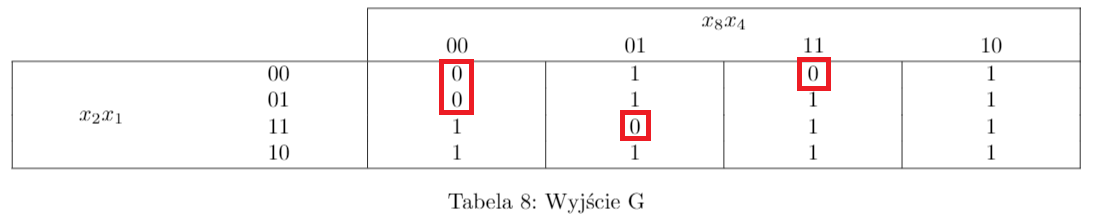
\includegraphics[width=18cm]{reports/img/Z1C_tab_8.png}\\
            \end{center}
            % \begin{center}
            %     \begin{table}[ht]
            %         \centering
            %         \begin{tabularx}{\textwidth}{|Y *{5}{Y|}}
            %             \cline{3-6} 
            %             \multicolumn{2}{c|}{} &
            %             \multicolumn{4}{c|}{$x_8x_4$}\\
                        
            %             \multicolumn{2}{c|}{} & \multicolumn{1}{c}{00} & \multicolumn{1}{c}{01} & \multicolumn{1}{c}{11} & \multicolumn{1}{c|}{10}\\
            %             \hline
                         
            %             \multirow{4}{*}{$x_2x_1$} & 00 & 0 & 1 & 0 & 1 \\
            %                                       & 01 & 0 & 1 & 1 & 1 \\
            %                                       & 11 & 1 & 0 & 1 & 1 \\
            %                                       & 10 & 1 & 1 & 1 & 1 \\
                        
            %              \hline 
            %         \end{tabularx}
            %         \caption{Wyjście G}
            %         \label{tab:my_label}
            %     \end{table}
            % \end{center}
            \FloatBarrier
            Skąd otrzymujemy (przez dopełnienie):
            $$G = (x_2+x_4+x_8)(\overline{x_1}+\overline{x_2}+\overline{x_4}+x_8)(x_1+x_2+\overline{x_4}+\overline{x_8})$$
            \FloatBarrier
            
            Za pomocą powyższych obliczeń wyprowadziliśmy minimalną funkcję logiczną opisującą niezależnie każde z wyjść układu dekodera w zależności od bitów liczby wejściowej. Spróbujmy poszukać zależności pomiędzy wyjściami, które pozwoliłyby nam dalej zminimalizować układ (zgodnie z intuicją, że jeśli przykładowo dwa segmenty wyświetlacza świeciłyby się zawsze w tych samych momentach, nie potrzebowalibyśmy dwóch niezależnych dekoderów dla obu z tych segmentów).             
            \begin{center}
                \begin{table}[ht]
                    \centering
                    \begin{tabularx}{\textwidth}{|Y *{9}{Y|}}
                        \cline{3-10} 
                        \multicolumn{2}{c|}{} &
                        \multicolumn{8}{c|}{EFG}\\
                        
                        \multicolumn{2}{c|}{} & \multicolumn{1}{c}{000} & \multicolumn{1}{c}{001} & \multicolumn{1}{c}{010} & \multicolumn{1}{c|}{011} & \multicolumn{1}{c}{100} & \multicolumn{1}{c}{101} & \multicolumn{1}{c}{110} & \multicolumn{1}{c|}{111}\\
                        \hline
                         
                        \multirow{4}{*}{BCD} & 000 & - & - & - & - & - & - & - & 1 \\
                                             & 001 & - & - & - & - & - & - & - & 1\\
                                             & 010 & - & - & - & - & - & - & - & -\\
                                             & 011 & - & - & - & 1 & - & - & 1 & 1/0\\
                                             & 100 & - & - & - & - & - & - & - & -\\
                                             & 101 & - & - & - & - & - & 1 & - & -\\
                                             & 110 & 0/1 & - & - & 1 & - & - & - & 1\\
                                             & 111 & - & 1 & - & - & - & 0 & 1 & 1\\
                         \hline 
                    \end{tabularx}
                    \caption{Opis stanów wyjścia A w zależności od pozostałych wyjść dekodera}
                    \label{tab:my_label}
                \end{table}
            \end{center}
            Niestety, podczas próby konstrukcji tablicy stanów opisującej stan wyjścia A w zależności od stanu pozostałych wyjść odkryliśmy, że nie istnieje deterministyczna funkcja opisująca taką zależność - znaleźliśmy dwie sytuacje, w których wyjście A przyjmuje różne wartości dla tych samych stanów pozostałych bramek. Oznacza to, że otrzymana w poprzednim punkcie zależność dla wyjścia A od bitów liczby wejściowej jest optymalna. \\
            Dla pozostałych wyjść układu, z wyjątkiem wyjścia F, również wskazać możemy takie sytuacje konfliktowe. Dla porządku wypiszmy je poniżej. 
            \begin{itemize}
                \item Dla złącza B gdy pozostałe wyjścia przyjmują wartość 1 (to jest dla liczb 1000 i 0110).
                \item Dla złącza C gdy złącze B przyjmuje wartość 0, a pozostałe złącza 1 (to jest dla liczb 1110, 0110).
                \item Dla złącza D gdy wszystkie pozostałe złącza przyjmują wartość 1 (to jest dla liczb 1010 i 1000).
                \item Dla złącza E gdy złącze B przyjmuje wartość 0, a pozostałe złącza 1 (to jest dla liczb 0101 i 0110).
                \item Dla złącza G gdy wszystkie pozostałe wyjścia przyjmują wartość 1 (to jest dla liczb 0000, 1000).
            \end{itemize}
            \newpage
            Nie udało nam się znaleźć konfliktu dla wyjścia F. Rozpiszmy zatem jego tabelę prawdy. 
            \begin{center}
                \begin{table}[ht]
                    \centering
                    \begin{tabularx}{\textwidth}{|Y *{9}{Y|}}
                        \cline{3-10} 
                        \multicolumn{2}{c|}{} &
                        \multicolumn{8}{c|}{DEG}\\
                        
                        \multicolumn{2}{c|}{} & \multicolumn{1}{c}{000} & \multicolumn{1}{c}{001} & \multicolumn{1}{c}{010} & \multicolumn{1}{c|}{011} & \multicolumn{1}{c}{100} & \multicolumn{1}{c}{101} & \multicolumn{1}{c}{110} & \multicolumn{1}{c|}{111}\\
                        \hline
                         
                        \multirow{4}{*}{ABC} & 000 & - & - & - & - & - & - & - & - \\
                                             & 001 & - & - & - & - & - & - & - & 1\\
                                             & 010 & - & - & - & - & - & - & - & - \\
                                             & 011 & 0 & - & - & - & - & - & - & 0 \\
                                             & 100 & - & - & - & 1 & - & - & 1 & 1 \\
                                             & 101 & - & - & - & - & - & 1 & - & 1 \\
                                             & 110 & - & - & - & - & - & - & - & 0 \\
                                             & 111 & 0 & 1 & - & 1 & - & 0 & 1 & 1 \\
                         \hline 
                    \end{tabularx}
                    \caption{Opis stanów wyjścia F w zależności od pozostałych wyjść dekodera}
                    \label{tab:my_label}
                \end{table}
            \end{center}
            Korzystając z powyższej tabeli wyprowadzić możemy zależność: 
            $$F = A(G+E) + A\overline{B}D + DE(\overline{B}+ABC)$$
            Uzyskaliśmy alternatywną zależność dla wyjścia F. Nie jest ona jednak realizowana za pomocą mniejszej ilości bramek logicznych, niż wskazana przez nas wcześniej zależność względem wejść układu.\\
            
            Tym samym pokazaliśmy, że otrzymujemy układ zbudowany z optymalnej ilości bramek logicznych. 
        
        \subsection{Projekt układu}
            \begin{center}
                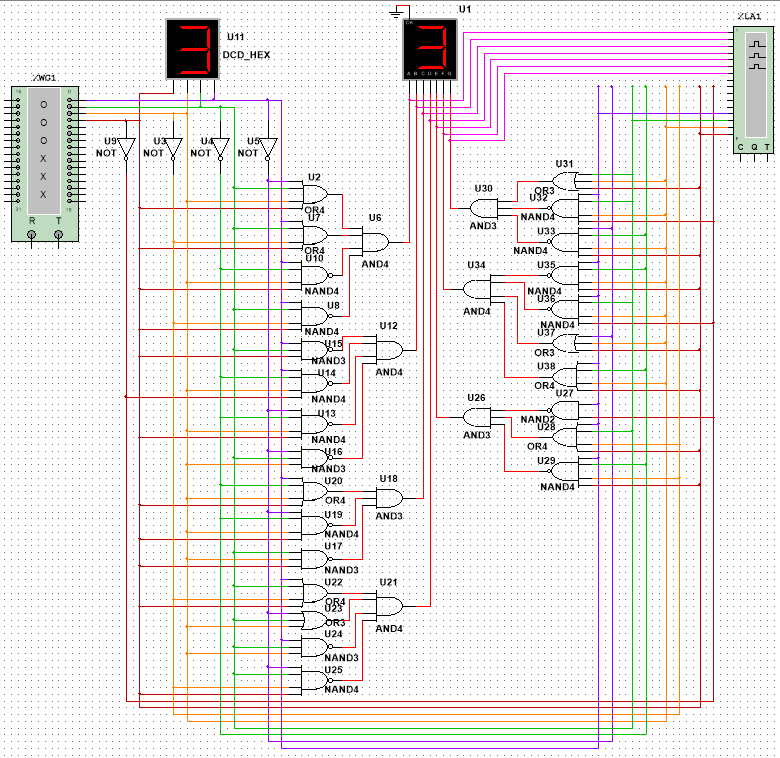
\includegraphics[height=18cm]{reports/img/Z1C_1.png}\\
            \end{center}
            W układzie jako źródło sygnału wykorzystano generator słów. Wyjścia odpowiadające za kolejne bity, w kolejności od najmniej do najbardziej znaczącego, oznaczono odpowiednio kolorami: fioletowym, zielonym, pomarańczowym i bordowym. \\
            Sygnał odpowiadający za kolejne wejścia wyświetlacza przetwarzany jest przy pomocy bramek logicznych, zgodnie z powyżej rozpisanymi formułami. Niektóre operacje alternatywy logicznej realizowane są poprzez użycie bramki NAND zgodnie z prawem de Morgana. \\
            Do wejścia układu dołączono wyświetlacz DCD\_Hex ze wbudowanym transkoderem dla zilustrowania poprawności działania układu.
        
        \subsection{Symulacja}
            Generator słów kierowany jest sygnałem wyzwalającym z wbudowanego zegara o częstotliwości 50HZ. Podaje on na wyjścia wszystkie liczby czterobitowe w cyklu. 
            \begin{center}
                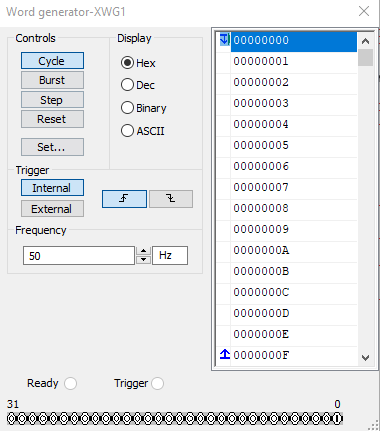
\includegraphics[height=9cm]{reports/img/Z1C_gen.png}\\
            \end{center}
            \begin{center}
                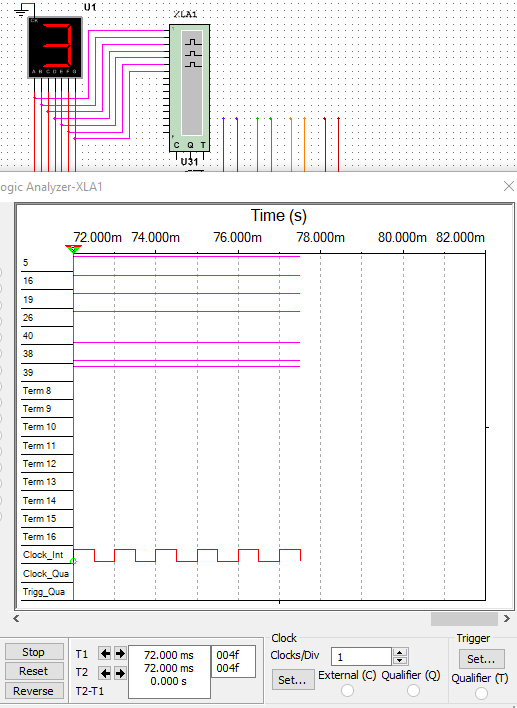
\includegraphics[height=9cm]{reports/img/Z1C_analize.png}\\
            \end{center}
            Za pomocą analizatora logicznego, oraz podłączonego wyświetlacza siedmiosegmentowego możemy stwierdzić poprawność działania dekodera.

        \subsection{Wnioski}
            Minimalizacja funkcji logicznych metodą Karnaugha pozwala  w sposób intuicyjny konstruować układy realizujące funkcje logiczne. Daje ona nam łatwość konstrukcji złożonych wyrażeń w sposób graficzny przy zapewnionej poprawności działania. W efekcie proces projektowania jest prostszy w porównaniu do próby minimalizacji klasycznego zapisu algebry booleowskiej.\\
            Znacząco usprawnia to projektowanie układów których działanie określone jest względem wielu zmiennych logicznych za pomocą wielu funkcji logicznych. Przykładem takiego układu jest transkoder na wyświetlacz siedmiosegmentowy.\\
            Zgodnie z prawem każdy sklep wyposażony musi być w kasę fiskalną. Taka kasa fiskalna wyświetla sumę cen wprowadzonych produktów za pomocą wyświetlacza zbudowanego z modułów siedmiosegmentowych. Każdy z takich modułów może być wyposażony w dekoder podobny do zaimplementowanego powyżej.


\end{document}
